\chapter{INTRODUÇÃO}\label{CAP:introducao}
O levantamento feito pelo Instituto Brasileiro de Geografia e Estatísticas (IBGE), em 2013, indicou que 6,2\% da população brasileira tem algum tipo de deficiência \citeonline{IBGE-2013}. O estudo mostra também que 1,3\% da população tem algum tipo de deficiência física. Da população com deficiência física, 46,8\% tem grau intenso ou muito intenso de limitações, nos casos extremos impossibilita a pessoa de realizar as atividades habituais.

O ininterrupto desenvolvimento de novas tecnologias, \textit{softwares} e \textit{hardwares} concebem uma ampla evolução nas estruturas sociais, corporativas e acadêmicas, porém existem áreas ainda pouco exploradas. Entre elas, é possível destacar a concepção das soluções baseadas em Tecnologia Assistiva (TA).

O conceito de TA, apesar de recente, pode ser definido como o conjunto de sistemas, tecnologias e inovações que permitem aumentar as habilidades funcionais de uma pessoa com algum tipo de deficiência e, desta forma, possibilitar sua inclusão. Segundo \citeonline{Bersch}, o objetivo da TA é proporcionar à pessoa com deficiência maior independência, qualidade de vida e inclusão social, através da ampliação de sua comunicação, mobilidade, controle de ambiente, habilidades de aprendizado, trabalho e integração com a família, amigos e sociedade.

O grande desafio de criar as condições necessárias à acessibilidade das Tecnologias da Informação e Comunicação (TICs) por pessoas com deficiência, transformando a interação desses usuários o mais simples possível, é presente dentro da área de Interação Humano-Computador (IHC). É evidente que as características humanas e os estilos de interação são fatores determinantes no modo como é feita a interação com as TICs através das tecnologias.

Tendo em vista os fatores já citados, as motivações pessoais e as áreas de interesse como TA, Visão Computacional (VC) e Processamento Digital de Imagens (PDI), motivou o desenvolvimento do VisiUMouse, que é  uma tecnologia que permite o uso de um computador por pessoas com algum tipo de deficiência física por meio do rastreamento dos movimentos dos olhos através da entrada de vídeo da \textit{webcam}, utilizando os conceitos e premissas da VC. Possibilitando o uso desta tecnologia para qualquer pessoa no mundo por meio de \textit{download} do \textit{Software} disponível em um repositório público e gratuito \footnote{http://www.visiumouse.com}.

Visão Computacional é a área da ciência que desenvolve teorias e métodos voltados à extração automática de informações úteis contidas em imagens \cite{prince2012computer}. O objetivo dessa ciência é criar e transmitir essas informações às máquinas de forma compreensível, segundo \citeonline{prince2012computer}.


%% REVDEIA 4: PEÇA PARA ALGUÉM LER TEU TRABALHO EM VOZ ALTA, FACILITA PARA ENCONTRAR OS ERROS , COMO POR EXEMPLO: Restando do trabalho.... esta irei alterar, mas não conseguirei fazer em todo
O restante do trabalho esta organizado da seguinte forma: o Capítulo \ref{CAP2} apresenta a fundamentação teórica, o Capítulo \ref{CAP3} descreve a Metodologia utilizada, o Capítulo \ref{CAP4} apresenta o desenvolvimento da aplicação desenvolvida, o Capítulo \ref{CAP5} apresenta a modelagem do VisiUMouse, o Capítulo \ref{CAP6} expõe os conceitos de Design utilizados,  o Capítulo \ref{CAP6-tecnilogias-utilizadas} apresenta as tecnologias utilizadas no desenvolvimento, o Capítulo \ref{CAP-tecnologia-visiumouse} demonstra como utilizar o VisiUMouse, o Capítulo \ref{CAP7} refere-se aos experimentos de avaliação realizados com o \textit{software} VisiUMouse e faz uma análise de seus resultados e o Capítulo \ref{CAP-consideracoes-finais-trabalhos-futuros} retrata as considerações finais.
%------------------------------------------------------------------


\chapter{FUNDAMENTAÇÃO TEÓRICA E MOTIVAÇÕES}\label{CAP2}
A evolução contínua e exponencial das tecnologias possibilitam cada vez mais a criação e melhorias de em vários âmbitos sociais, digitais, acadêmicos e profissionais. Para isso cada pessoa tem acesso a um arsenal de conhecimento imensurável, na \textit{internet}, como a grande quantidade de artigos e pesquisas acadêmicas publicados diariamente e o desenvolvimento e distribuição continuo de \textit{softwares} de código aberto. É evidente o crescimento das possibilidades em todas as áreas de conhecimento com a revolução da informação, representado um novo modelo mundial para todas as pessoas.


\section{TECNOLOGIA ASSISTIVA}\label{Sub:ta-brasil}
Tecnologia Assistiva pode ser considerada como todos os recursos e serviços que contribuem para proporcionar ou ampliar as habilidades funcionais de pessoas com deficiência e consequentemente promover vida independente e inclusão. O termo TA, que é uma expressão nova, e se refere a um conceito ainda em pleno processo de construção e sistematização. A utilização de recursos de TA, entretanto, remonta aos primórdios da história da humanidade ou até mesmo da pré-história. Qualquer pedaço de pau utilizado como uma bengala improvisada, por exemplo, caracteriza o uso de um recurso de TA. \cite{galvao2009tecnologia-UPPERCASE}.

As pessoas com deficiência motora (membros superiores) encontram, ainda, grande dificuldades em utilizar um computador pessoal, pelo fato de que os dispositivos padrão de interação são controlados basicamente apenas pelo movimento das mãos. Este motivo incapacita a utilização de dispositivos de entrada tradicionais, como o \textit{mouse} e teclado. Para essas pessoas uma tarefa simples de navegar na \textit{internet} para estudar se torna um desafio intangível, atenuado apenas pelos poucos, e caros, dispositivos de TA disponíveis no mercado. São poucas as tecnologias que dão suporte a casos onde o usuário tem apenas o controle do movimento da cabeça. Em muitos dos casos de deficiência motora, como por exemplo a ELA (Esclerose Lateral Amiotrófica), deficiência causada por acidente ou paralisia cerebral, essas pessoas possuem as faculdades mentais intactas.


%% REVDEIA 6: DEI UMA REESCRITA NESTE PARÁGRAFO ABAIXO
Estes fatos permitem que essas pessoas interajam com o seu ambiente de outras maneiras não convencionais, com os movimentos ainda restantes, e como os movimentos da cabeça são, os que nestes casos, permanecem funcionais, são movimentos que podem ser explorados para uma possível maneira de interação com o computador, isto é, o precisa haver um dispositivo de TA, de entrada, que capte os movimentos da cabeça (como rotação e flexão) e seus elementos, como boca, nariz e olhos, além da fala. 

Considerando estes fatos podemos citar três tipos de entrada, alternativos:
\begin{enumerate}
\item A entrada de vídeo, onde o usuário estará disposto na frente de uma câmera como a \textit{webcam}.
\item A entrada de áudio, onde o usuário vai precisar ter um microfone.
\item E por fim a entrada de contato físico, onde o usuário vai precisar apertar botões ou switchs.
\end{enumerate}

% * <tsixav@gmail.com> 2018-04-17T01:00:16.483Z:
% 
% Ainda nessa seção da para falar dos nives de TA: baixo, medio e alto, como o rafa comentou no audio.
% 
% ^.


\section{VISÃO COMPUTACIONAL}\label{Sub:vc}

Visão Computacional é uma subárea da Inteligência Artificial (IA) que tem como objetivo dar significado as imagens digitais com base em análise. Esta análise procura extrair algum conhecimento da representação matricial das imagens, segundo \citeonline{prince2012computer}. 

São alguns exemplos referentes a área de VC: 
\begin{itemize}
\item A estimativa de segmentação e de movimento.
\item Reconstrução de fotografias para a criação de modelos tridimensionais, como rostos humanos.
\item Análise de segmentação.
\item Reconhecimento de objetos orgânicos e inorgânico.
\item Rastreamento de alvos.
\end{itemize}

Estes desafios tornam-se complexos pelo fato das imagens digitais serem apenas visíveis para o computador, frequentemente são estrutura de dados no formato de matrizes de distribuição de pontos e também pelo fato de não armazenarem informações sobre a cena representada pela imagem, isto é meta dados, de acordo com \citeonline{prince2012computer}.

Um dos grandes desafios da área de VC é a detecção e rastreamento de alvos, principalmente por sua aplicação em sistemas de vigilância de vídeo, análise de atividade humana, monitoramento de tráfego urbano e rural, rastreamento de animais e robótica autônoma. A análise de atividade humana ganha destaque quando possibilita uma automatização ou facilitação de uma atividade, como utilizar o computador todos os dias \cite{alaya2012multipeople-UPPERCASE}.

Visando solucionar os problemas citados anteriormente, a área de VC utiliza de reconhecimento de padrões, aprendizado de máquina (\textit{machine learning}), Geometria Projetiva (GP), PDI e teoria dos grafos \cite{prince2012computer}. É comumente visto em aplicações de redes sociais como o reconhecimento de amigos em uma foto do Facebook ou em zoom automático em fotos com muitos rostos, a Figura \ref{fig:exemplo-vc} ilustra um exemplo de múltiplos reconhecimentos de rostos (retângulos verdes) em um mesmo instante.
%[htbp]
\begin{figure}[H]
\caption{Exemplo de aplicação de Visão Computacional para o reconhecimento de rostos.}
\centering 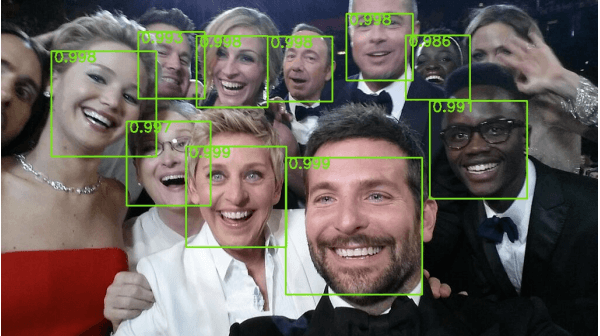
\includegraphics[scale=0.6]{img/figura-1.png}
 
{\fontsize{11}{11}\selectfont \textbf{Fonte:} Elaborada pelo autor.}
\label{fig:exemplo-vc}
\end{figure}

Considerando três tipos de entrada de dados comuns, como vídeo, áudio e toque é possível analisar que a entrada de vídeo possibilita uma interseção mais natural, considerando que o movimento da cabeça deve ser similar ao movimento da mão quando um usuário sem deficiência utiliza o \textit{mouse}.

Um vídeo pode ser considerado um conjunto de imagens digitais, que é uma representação numérica de uma imagem bidimensional, em forma binária, tornando possível o armazenamento, transferência, processamento ou reprodução por meios eletrônicos. Existe dois tipos de imagens, as imagens de rastreio (ou \textit{raster}) e as imagens do tipo vetorial. \cite{parker2010algorithms-UPPERCASE}.

As imagens de rastreio são representadas de forma matricial pelo computador, onde há uma correspondência 'bit-a-bit' da matriz que representa a imagem como o que está sendo reproduzido de fato na tela. A resolução de uma imagem define a sua matriz, então uma imagem de 1024x720 tem 737280 posições em uma matriz. 

As matrizes deste tipo não possuem nem um tipo de dados adicionais como o que existem na imagem ou que tipo de objetos ele representa. A representação e extração destes dados é tarefa da área de VC, que tem como objeto dar significado semântico para imagens digitais através do processamento delas, de acordo com \citeonline{prince2012computer}. Uma das técnicas para detectar objetos em uma imagem digital é o algoritmo de Viola-Jones.

\subsection{Conceito de Viola-Jones}

O algoritmo de Viola-Jones para a identificação de objetos é um algoritmo proposto para o reconhecimento de objetos em imagens digitais, e tem como característica o alto desempenho de processamento e o alto índice de assertividade, podendo chegar até a 99,7\% dependendo do número de etapas treinadas, acurácia do classificador do objeto para qual foi treinado, segundo \citeonline{viola2001rapid}. O qual trabalha com algoritmos em cascata que se utiliza de padrões e características chamados de \textit{haar features}. Estas características são organizadas em uma estrutura de árvore em XML (\textit{Extensible Markup Language}).

\subsection{Machine Learning}

\textit{Machine Learning} é utilizada para reconhecer padrões em um grupo de dados, como exemplo podemos citar os padrões que boa parte dos rostos humanos apresentam. Segundo \citeonline{samuel1959some}, podemos definir \textit{Machine Learning} como o campo de estudo que dá aos computadores a habilidade de aprender sem serem explicitamente programados. O aprendizado explora o estudo e construção de algoritmos que podem aprender de seus erros e fazer previsões sobre dados, esses algoritmos operam construindo um modelo a partir de entrada de dados amostrais com o objetivo de fazer previsões ou decisões guiadas pelos dados.

\chapter{METODOLOGIA}\label{CAP3}

Podemos dizer que metodologia é a explicação detalhada e exata de toda ação desenvolvida no (caminho) do trabalho. É a explicação do tipo de pesquisa, dos instrumentos utilizados, do tempo previsto, da equipe de pesquisadores e da divisão do trabalho, das formas de tabulação e tratamento dos dados, enfim, de tudo aquilo que se utilizou no trabalho de pesquisa, de acordo com \citeonline{miner2012mapreduce}.

O objetivo geral do trabalho é desenvolver uma TA com base em VC que permita uma pessoa com deficiência físico motora (principalmente os membros superiores) consiga controlar o seu computador apenas com o movimento da cabeça (usando os olhos como pontos de referência), através da manipulação do movimento e cliques do \textit{mouse}.


Entre os objetivos específicos podemos citar: 
\begin{enumerate}
\item O desenvolvimento do VisiUMouse para multiplataformas.
\item Desenvolvimento do site do VisiUMouse onde será possível fazer o \textit{download} dele de forma gratuita, entre outras funcionalidades.
\item Garantir que os mecanismos de busca dos navegadores modernos achem ele pela busca da palavra "VisiUMouse".
\item Desenvolver um instalador.
\item Garantir que o VisiUMouse tenha as principais funcionalidades de um \textit{mouse} tradicional.
\item Criar uma interface de configuração amigável e de utilização simples.
\end{enumerate}

Para isto foi necessário fazer uma pesquisa de possíveis TA, estudos relacionados e testes avaliativos para determinar a viabilidade do desenvolvimento dos objetivos propostos.
    
\section{TRABALHOS RELACIONADOS}\label{Sub:trabalhos-relacionados}

Existem vários tipos de  \textit{softwares} de TA, e a seguir são apresentados alguns. Parte deles são utilizados para a comunicação com outras pessoas, porém existem outros que tem como objetivo a independência, o qual permite que seus usuários exerçam atividades sozinhos ou com a mínima ajuda possível, ou seja, torna o usuário mais autônomo.

%Foi feito um Mapeamento Sistêmico com cerca de 2000 artigos, que foram utilizados como referência para o levantamento dos Trabalhos Relacionados. \cite{da2018best-UPPERCASE}.

Existem diversos projetos, produtos e estudos em TA, baseados na VC, que utilizam-se de \textit{softwares} para detecção de objetos através de uma \textit{webcam} \cite{ramos2016letras} , \cite{gips2000camera}, \cite{bian2016facial}, \cite{marnik2014blinkmouse}. A detecção dos movimentos nesses projetos é feita através de uma entrada de vídeo que rastreia várias partes do corpo humano, sendo que a mais comum é o rastreamento de movimentos da cabeça (\textit{video-based}). \cite{al2013eye-UPPERCASE}. 

Um dos objetivos de análise desses trabalhos é não depender de dispositivos de alto poder computacional, utilizando Tecnologias disponíveis no próprio computador. Das soluções \textit{video-based} a mais adotada é o \textit{software} CameraMouse \cite{gips2000camera} que frequentemente é usado como base de pesquisas e de comparações, como em Kurauchi \cite{kurauchi2015hmagic}. A seguir são apresentados um resumo de alguns dos \textit{softwares} difundidos no meio.

\subsection{CameraMouse}
O \textit{software} CameraMouse é capaz de capturar o movimento dos olhos ou qualquer outra parte do corpo com que se queira manipular o \textit{mouse} do computador. Ele foi desenvolvido para trabalhar com a plataforma Windows e seu funcionamento se dá através dos recursos do \textit{webcam}. O programa foi desenvolvido para ajudar as pessoas com deficiência e o principal público-alvo deste \textit{software} são as pessoas que não têm controle confiável das mãos, mas que podem executar movimentos com a cabeça \citeonline{gips2000camera}.

Dentre os softwares similares este é o mais semelhante a Tecnologia VisiUMouse, usando dos mesmos conceitos e princípios da VC. A Figura \ref{fig:camera-mouse} apresenta a tela inicial do CameraMouse, o quadrado pequeno na cor verde posicionado no nariz da pessoa representa a área que o usuário selecionou para o \textit{software} rastrear, forçando o usuário estar sempre na mesma posição, podendo apenas mover sua cabeça em inclinar para os lados, forçando o usuário a fazer movimentos espelhados  e assim causando um maior esforço do usuário. O CameraMouse não possibilita usar a inclinação da cabeça para controlar o \textit{mouse}, isto é, para o usuário mover o ponteiro ele preciso imaginar que na tela do computar existe um espelho e que ele deve posicionar o quadrado verde na área que deseja.

\begin{figure}[ht]
 \caption{Tela inicial do Software CameraMouse.} 
\centering 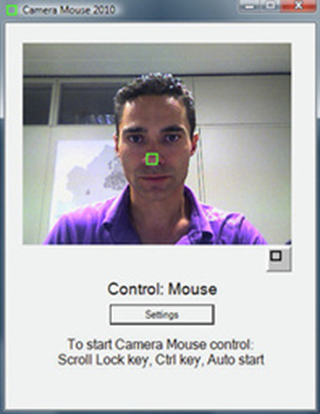
\includegraphics[scale=1]{img/camera-mouse.png}

{\fontsize{11}{11}\selectfont \textbf{Fonte:} Elaborada pelo autor.}
\label{fig:camera-mouse}
\end{figure}

\subsection{HeadDev}

O projeto HeadDev \citeonline{alvesferramentas} é semelhante ao CameraMouse, porém faz o rastreamento apenas dos movimentos da cabeça, não permitindo configurar o objeto que o \textit{software} deve rastrear. Seu funcionamento também utiliza a técnica de espelhamento.

HeadDev é um software gratuito para IHC sem o uso das mãos, cabos, sensores ou outro dispositivo. A interação é feita com uma \textit{webcam} USB padrão, que reconhece os movimentos do rosto. Ele destina-se a pessoas com deficiência motora grave (esclerose lateral amiotrófica, esclerose múltipla, paralisia cerebral, lesão medular e distrofia muscular), porque o sistema só utiliza os movimentos do nariz ou face como ponteiro do \textit{mouse} em um teclado virtual na tela do computador para fazer os eventos de um \textit{mouse}.

\subsection{Facial Mouse}

Facial Mouse é uma interface de IHC para as pessoas com tetraplegia baseada em uma câmera de profundidade de infravermelho monocular. A posição do nariz junto com a boca é detectado para o controle e navegação do cursor do \textit{mouse}. O algoritmo utilizado para rastrear é baseado em uma árvore melhorada de decisão aleatória que é capaz de detectar a informação facial de forma eficiente e com precisão. Com isso é possível uma experiência melhor para o usuário, tornando mais confortável o alcance do movimento do nariz para o movimento do cursor através de uma função não-linear. A câmera de profundidade infravermelha permite o sistema ser independente de iluminação e mudanças de cor tanto o fundo e no rosto humano, o que é uma vantagem crítica sobre as opções baseadas em câmera RGB \citeonline{bian2016facial}.

\subsection{Facial Human-Computer Interface}

Já o \textit{softwares} Facial Human-Computer Interface \citeonline{antunes2016intelligent}, tem como objetivo aplicar o modo de interação feita pelo CameraMouse, refinando a funcionalidade do clique, principalmente nos requisitos de precisão e configuração.

O Facial Human-Computer Interface é um sistema com IHC, que permite uma comunicação mais natural com as máquinas, seu publico alvo são pessoas idosas e deficientes. Ele apresenta um sistema baseado em visão e recurso para detecção de piscadas voluntárias longas e interpretação de padrões de piscada para comunicação entre homem e máquina. Complementado pelo mecanismo de detecção de múltiplos piscadas de olho, além disso oferece uma solução completa para a construção de dispositivos de entrada inteligentes com viva voz. A técnica utilizada para rastrear utiliza câmeras automáticas que permitem rastrear as características do nariz, sobrancelhas e a posição da cabeça de forma robusta e precisa nas coordenadas 2D e 3D. Esse rastreamento e monitoramento permitem que o usuário forneça dados para a máquina do computador e acesse todo o sistema de uma maneira livre, de acordo com \citeonline{parmar2012facial}. 


\section{OBJETIVO}\label{sub:objeto}

Baseado nos trabalhos relacionados percebe-se a utilização dos conceitos de VC e o uso da OpenCV, com a técnica de espelhamento do movimento e rastreamento da face principalmente. 



\textbf{Nesse contexto o VisiUMouse tem como um dos objetivos implementar uma técnica de movimento alternativa, batizada de Técnica de Zona Neutra e de Movimento (TZNM) \citeonline{xavier2017visiumouse}, com o rastreamento dos olhos para o controle do ponteiro, facilitando uma implementação futura de clique pelo piscar dos olhos e \textit{Eye Tracking}.}


%% REVDEIA 11: AQUI TAMBÉM ACHO QUE DEVERIA IR PARA O CAPÍTULO DO VISIUMOUSE 

\section{VIABILIDADE}\label{Sub:viabilidade}

Com a crescente evolução das áreas de IA é evidente o aumento de ferramentas e estudos que colaboram para a criação e implementação de novas aplicações. Uma subárea da IA que vem ganhando destaque é a VC que tem como foco extrair significado as imagens virtuais com base em análise e estudo de padrões.

Com a evolução da VC possibilitou a criação de novas aplicações, toda atividade humana que tinha como base a visão pode ser transformada em uma aplicação de VC. Grandes inovações nas áreas de saúde e Astronomia com a ajuda desta área agora são possíveis, por exemplo. Atualmente é possível utilizar esta área para a busca de estruturas estranhas em imagens de exames de tomografia. 
    
O potencial e a evolução da VC perpetuam o aumento de novos estudo e ferramentas. OpenCV é uma biblioteca grátis e multiplataforma, isto é compatível com múltiplos Sistemas Operacionais e Linguagens de Programação, como Java e C, ela foi desenvolvida pela Intel Corporation, que implementa diversos módulos e cerca de 350 algoritmos de VC, e atualmente está presente em diversos \textit{software} e estudos, tornando as aplicações de VC mais acessíveis.  

Os fatores apresentados manifestam as possibilidades de criação de aplicações com base em VC, grande parte deste cenário é possível graças a biblioteca OpenCV que é uma biblioteca de código aberto e compatível com os principais Sistemas Operacionais e Linguagens de Programação do mercado. Estes fatores determinam a escolha dela e da Linguagem de Programação Java para o desenvolvimento do trabalho. Assim como a maioria das Linguagens de Programação a Java não gera custos.

O trabalho proposto tem como público-alvo pessoas com algum tipo de deficiência motora ou física, que possuem o movimento da cabeça e com a capacidade cerebral preservada.

Os fatores apresentados e a experiência adquirida em outros projetos relacionados com acessibilidade e TA evidenciam aspectos para a viabilidade do trabalho apresentado. Entre as experiências podemos citar a quantidade de usuários com deficiência físico motora no Brasil e na região de Pelotas; de instituições que amparam esses usuários as quais podem ser abordadas diretamente para apresentar O VisiUMouse; que boa parte desses usuários não estão presentes diretamente na sociedade.

\section{METODOLOGIA DE DESENVOLVIMENTO}\label{Sub:metodologia-desenvolvimento}
Para o desenvolvimento desse trabalho foi utilizado o método de Design Centrado no Usuário (DCU), de acordo com \cite{GREENHOUSE2010}, a metodologia DCU não é um estilo de design, mas sim um processo para projetar e desenvolver produtos que se baseiam em informações sobre as pessoas que vão utilizá-las, uso de resultados de pesquisas e dados sobre habilidades cognitivas, capacidades físicas e limitações, necessidades sociais e os requisitos de tarefas com o objetivo de fornecer soluções para aplicações que sejam de acesso universal, independentemente de idade ou habilidade. 

Além disso foi utilizado a Metodologia Ágil SCRUM, nele os projetos são divididos em ciclos chamados de \textit{Sprints}. O \textit{Sprint} representa um \textit{Time Box} dentro do qual um conjunto de atividades deve ser executado. O SCRUM foi utilizado principalmente para organizar a prioridade das \textit{Sprints} relacionadas ao desenvolvimento, para garantir as datas de entrega e a organização do tempo disponível, segundo \citeonline{miner2012mapreduce}.

Para realizar os objetos desse trabalho, todo desenvolvimento do \textit{software} do VisiUMouse foi organizado em 3 ciclos: \textbf{Validação}, \textbf{Experimento} e \textbf{Melhoria}. A \textbf{Validação} foi ciclo inicial da criação da solução e tinha como objetivo validar a solução proposta, para validar foi criado um MVP, que tinha como principal funcionalidade o rastreamento dos olhos e o controle do \textit{mouse}; O \textbf{Experimento} teve como objetivo comprovar seu funcionamento, de uma tecnologia que permite o controle do \textit{mouse} apenas com o movimento da cabeça, além de levantar possíveis melhorias, como um autoajuste dos parâmetros de rastreamento e otimizar os algoritmos de processamento de vídeo; O último ciclo, \textbf{Melhoria},  compreendeu em implementar as melhorias levantadas no ciclo de \textbf{Experimento}, e após disponibilizar uma versão do \textit{software} do VisiUMouse no site oficial "www.visiumouse.com".


\chapter{VISIUMOUSE}\label{CAP4}
VisiUMouse é um projeto de VC com o objetivo de ajudar pessoas com algum tipo de deficiência físico motora a utilizar o computador de maneira simples e fácil apenas com do movimento da cabeça, usando os olhos como referência. Permitindo a substituição do \textit{mouse} comum por uma nova IHC adequada e configuráveis. O rastreamento dos olhos do usuário é sutil e não causa nenhum desconforto, para usuários que não podem usar dispositivos tradicionais de entrada de computador, como teclado, \textit{mouse} e teclado. Este tipo de tecnologia tem outro diferencial que é desnecessário um \textit{hardware}, sensor, sinal conectado no usuário.

\section{Arquitetura}\label{Sub:funcionamento-visiumouse}
VisiUMouse é um projeto que tem como objetivo principal a utilização de computadores pessoais (PC) exclusivamente com o movimento da cabeça, isto é possível com base na captura de vídeo feita pelo \textit{webcam} do usuário e o processamento dos dados do vídeo recebidos, e com o uso de algoritmos de rastreamento de objetos e \textit{Machine Learning} é possível reconhecer a posição atual dos olhos do usuário. 

A Figura \ref{fig:projeto-diagrama-alto-nivel} apresenta um diagrama de alto nível do funcionamento do VisiUMouse, do lado direito podemos ver o "Usuário" disposto na frente da "Webcam"; a \textit{webcam} é responsável por capturar vídeo do "Usuário"; para cada captura (ou \textit{frame}) do vídeo é enviado um conjunto de dados para o VisiUMouse, esse processo está demonstrado em "entrada de dados";  após a leitura dos dados é iniciado o processo de rastreamento dos olhos, representado por "rastrear olhos"; em seguida ao rastreamento é feita uma análise que interpreta o movimento/deslocamento dos olhos do usuário, como podemos ver em "interpretar movimento"; e por fim o movimento dos olhos do usuário é retratado no controle do movimento do \textit{mouse}, representado por "controle mouse".

\begin{figure}[htbp]
\centering
\caption{Diagrama de alto nível do VisiUMouse.}
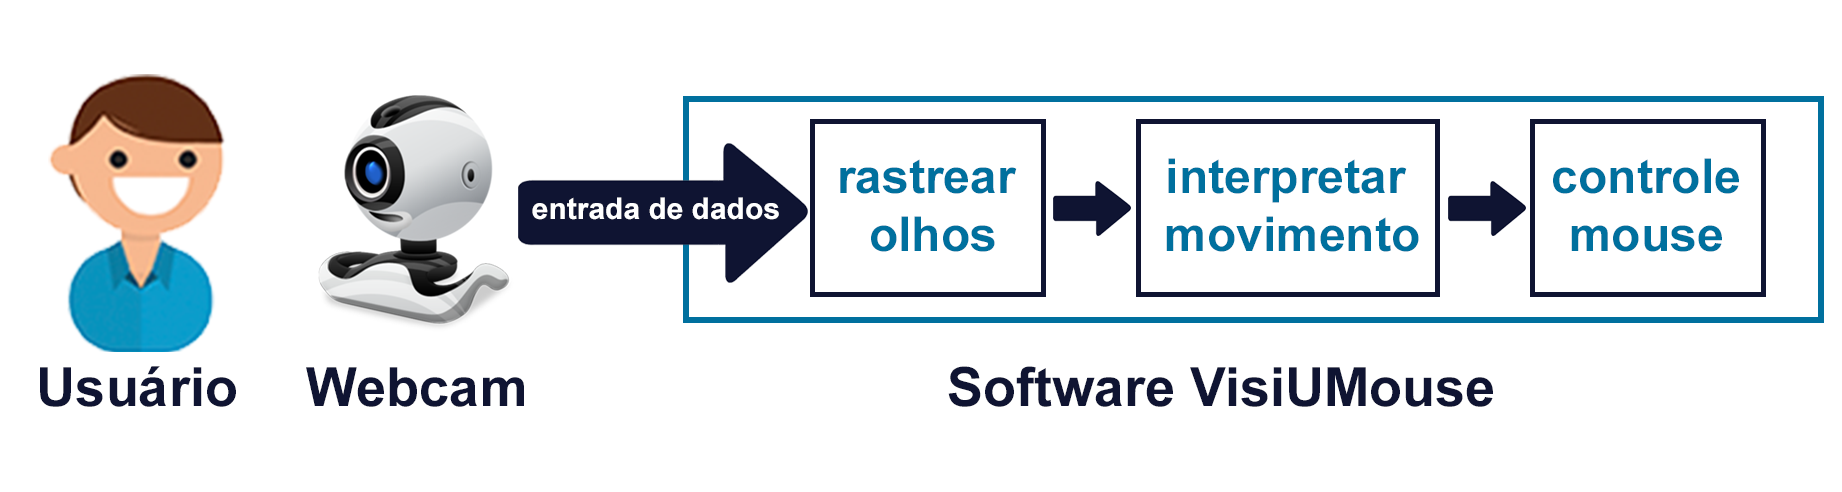
\includegraphics[scale=.25]{img/projeto-diagrama-alto-nivel.png}

{\fontsize{11}{11}\selectfont \textbf{Fonte:} Elaborada pelo autor.}
\label{fig:projeto-diagrama-alto-nivel}
\end{figure}

O processo de \textit{Machine Learning} é utilizado para reconhecer padrões de formas de objetos, neste caso foi para rastrear olhos humanos, para isso foi necessário utilizar um banco de dados com grande volume de imagens de olhos que gerou um arquivo XML com estes padrões. Com o arquivo XML com os padrões foram utilizados os conceitos do algoritmo de Viola-Jones para fazer o processo de rastreamento \cite{viola2001rapid}. Este arquivo XML contém os padrões e características são chamados de \textit{haar features}, que são uma lista de características invariantes de um objeto.

Os objetos procurados pela estrutura de detecção universalmente envolvem as somas de pixeis de imagem dentro de áreas retangulares, estes valores são comparados com os valores dos estágios do arquivo \textit{haar fea-tures}, e assim determinar se a área examinada da imagem possui ou não o objeto que pretende detectar. A Figura \ref{fig:viola-jones-ret} apresenta o processo de somas de pixeis da imagem que está sendo trabalhada, as somas são feitas dentro dos retângulos. 

\begin{figure}[H]
\caption{Algoritmo de Viola Jones.} 
\centering 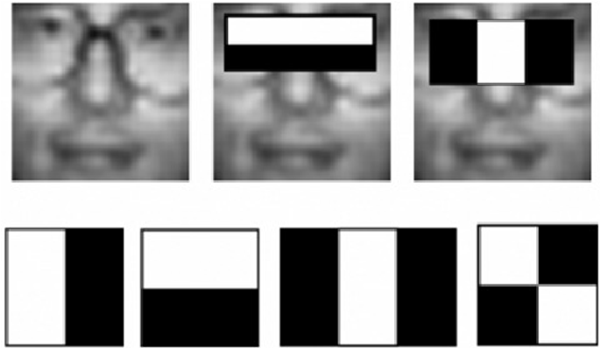
\includegraphics[scale=0.6]{img/viola-jones-ret.png}

{\fontsize{11}{11}\selectfont \textbf{Fonte:} Elaborada pelo autor.}
\label{fig:viola-jones-ret}
\end{figure}

Aplicação de rastreamento dos olhos foi desenvolvida usando a linguagem de programação Java, esta linguagem oferece um arsenal de bibliotecas para PDI e o suporte a desenvolvimento de sistemas multiplataforma, isto é, funciona em diferentes Sistemas Operacionais. 

Normalmente os processos de rastreamento são feitos em um processador responsável pela renderização de gráficos em tempo real. Este tipo de processador é chamado de \textit{Graphics Processing Unit}, também conhecido como GPU.

Genericamente o processamento da imagem contém 3 estágios: Captura, Análise e Compressão da Imagem. A \textbf{Captura} trata da aquisição dos dados de entrada de vídeo; a \textbf{Análise} trata do reconhecimento do objeto alvo. Para o reconhecimento é necessário um conjunto de padrões do alvo, esse processo é nomeado de Treinamento e é responsável por gerar um arquivo XML que contém características e padrões dos objetos alvos. A Classificação é o processo final que define se um determinado pedaço da imagem contém o objeto que pretende detectar. A \textbf{Compressão da Imagem} é o processo feito para reduzir a redundância dos dados, de forma a armazenar ou transmitir esses mesmos dados de forma eficiente, de acordo com \citeonline{rolim2008sistema}.

Com os conceitos do algoritmo de Viola-Jones e as bibliotecas de suporte a PDI foi possível desenvolver o VisiUMouse, o qual tem como característica principal o reconhecimento e rastreio dos olhos do usuário, para  que ele controle o \textit{mouse}. O processo de movimento dos olhos e o movimento do ponteiro do \textit{mouse} é dado em dezenas de milissegundo, este valor depende da GPU do computador do usuário. A Figura \ref{fig:visiumouse-1} mostra o funcionamento do rastreando dos olhos do usuário.
\begin{figure}[H]
\centering
\caption{Tela de captura de vídeo do VisiUMouse.}
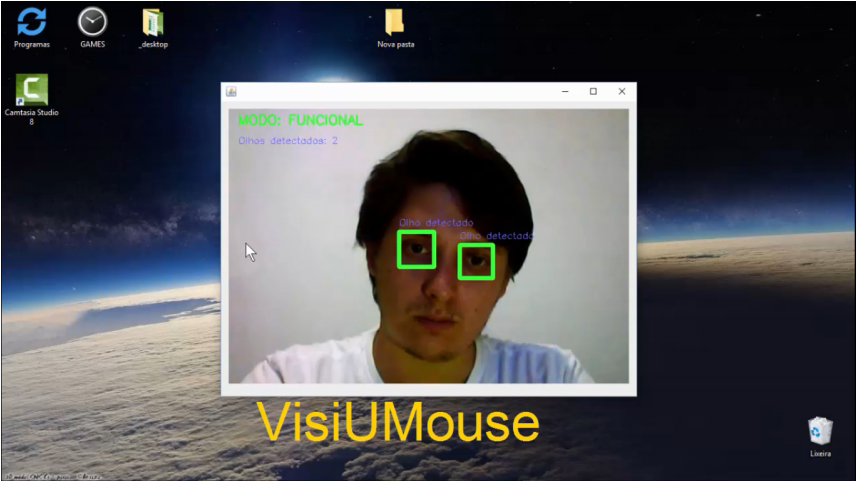
\includegraphics[scale=.4]{img/visiumouse-1.png}

 {\fontsize{11}{11}\selectfont \textbf{Fonte:} Elaborada pelo autor.}
\label{fig:visiumouse-1}
\end{figure}

O VisiUMouse tem seu funcionamento baseado no movimento da cabeça/face, usando os olhos como ponto de referência e a Técnica de Zona Neutra e de Movimento (TZNM). A medida do deslocamento dos olhos é feita através do processamento das posições anteriores, ou seja, se a medida for superior a configurada é feita a movimentação do ponteiro (zona de movimento da TZNM), se for menor o ponteiro permanece parado (zona neutra da TZNM). Para processar para qual lado o cursor deve ir é verificada a posição dos olhos em relação às linhas (ilusórias) vermelha e verde, como pode ser visto na Figura \ref{fig:funcionamento}.

\begin{figure}[H]
\caption{VisiUMouse: telas de rastreamento e processamento do deslocamento dos olhos.}
\centering 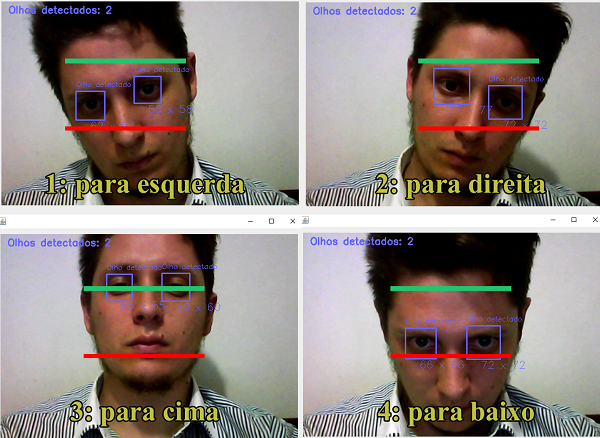
\includegraphics[scale=.8]{img/funcionamento2.png}

{\fontsize{11}{11}\selectfont \textbf{Fonte:} Elaborada pelo autor.}
\label{fig:funcionamento}
\end{figure}

Para determinar a direção do movimento do ponteiro é feita uma comparação com a posição dos olhos em relação às linhas verde e vermelha. Por exemplo, se o olho direito estiver próximo da linha verde e o olho esquerdo próximo da linha vermelha, indica que o usuário está com a cabeça inclinada para esquerda e que o cursor do \textit{mouse} deve ir para o mesmo lado, como mostrado na Figura \ref{fig:funcionamento} (1: para esquerda). Também é possível fazer movimentos para direita, para cima e para baixo (vide Figura \ref{fig:funcionamento}), além da combinação desses movimentos, tornando possível realizar movimentações em diagonal. No momento em que o movimento do cursor do \textit{mouse} se inicia, o usuário não precisa mais deslocar os olhos para manter o movimento, ele apenas precisa permanecer na mesma posição, podendo tornar o controle do \textit{mouse} menos cansativo, e assim evitando o desgaste físico do usuário \footnote{Foi disponibilizado um vídeo com o funcionamento básico do VisiUMouse, em: http://visiumouse.com/\#funcionamento}. 




%%ALIÁS, FARIA MUITO MAIS SENTIDO SE ESTAS OBSERVAÇÕES E A TABELA COMPARATIVA ESTIVESSE EM TRABALHOS RELACIONADOS
\subsection{Comparação com Soluções Análogas}\label{Sub:tabela-comparativa}

A área de TA apresenta um número significativo de tecnologias que permitem o melhor uso de um computador e comunicação, algumas dessas tecnologias tem como objetivo ajudar na formulação de frases através de um teclado com imagens, que representam palavras comuns, como: comer, água, banheiro, música etc. Outra parte dessas tecnologias tem como objetivo viabilizar o uso do Computador sem ajuda de outras pessoas, geralmente essas tecnologias apresentam controles de acionamento mecânico como grandes pedais ou palancas. Entra elas ainda podemo citas as que utilizam poder computacional, como as que permite o uso do computador apenas com o movimento da cabeça, geralmente a leitura do movimento é feito por um  entrada de vídeo que filma e interpreta seus movimentos.

A Tabela \ref{tabela-comparativa} apresenta uma comparação entre os \textit{softwares}: VisiUMouse, CameraMouse e FacialMouse; os quais apresentam algumas semelhanças como: \textit{webcam} como entrada de vídeo, uso da biblioteca OpenCV e do algoritmo de Viola-Jones. O CameraMouse é usado em diversas pesquisas, tendo mais de mil resultados no Google Acadêmico. O FacialMouse apresenta um refinamento em suas funcionalidades comparado ao CameraMouse. O CameraMouse e FacialMouse são um dos poucos que estão disponível para \textit{download}, é difícil o acesso as TA, grande parte são presente apenas em artigos acadêmicos, são poucas as que estão disponíveis para o publico, além disso elas ainda não difícil de encontrar, algumas por terem nomes genéricos outras por terem sites não ranqueado em motores de busca como Google.


A Tabela \ref{tabela-comparativa} apresenta 6 atributos de comparação:
\begin{enumerate}
\item \textbf{Clique por Tempo}: os dispositivos de TA com base em vídeo geralmente utilizam a técnica do clique do \textit{mouse} para simplificar o uso, esta técnica consiste em deixar o cursor do \textit{mouse} parado por um determinado tempo para gerar o clique na mesma posição que o curso está. Apesar de o clique por tempo ser comumente utilizado pode influenciar no desempenho do usuário em executar tarefas no computador que necessitam ser rápidas, como jogos. O VisiUMouse faz o rastreamento dos olhos permitindo implementar uma funcionalidade de clique pelo piscar dos olhos. 

\item \textbf{Tipos de Cliques}: este atributo representa a variedade de tipos de clique e funcionalidade do \textit{mouse} que a tecnologia apresenta, entre eles estão o clique primário (comumente o botão esquerdo do \textit{mouse}), clique secundário (comumente o botão direito do \textit{mouse}), a funcionalidade de arrastar etc.

\item \textbf{Multiplataforma}: característica de um sistema funcionar igualmente em diferentes plataformas (Sistemas Operacionais).

\item \textbf{Tipo de Movimento}: atributo que define como o movimento do cursor é feito em ralação ao objeto rastreado. As TA apresentadas utilizam o movimento espelhado que pode ser determinado por um reflexo do movimento do objeto rastreado no moimento do cursor do \textit{mouse}, apesar de ser intuitivo pode causar um desgaste físico extra na região do pesco e tornar inviável para pessoas que tenham menos mobilidade com a cabeça. A TZNM apresenta uma solução alternativa para o movimento do cursor do \textit{mouse} possibilitando um desgaste físico menor e o movimento por toda a tela do computador com uma menor mobilidade da parte do usuário.

\item \textbf{Objeto Rastreado(s)}: atributo que define qual objeto da cabeça do usuário é rastreado, ou seja, o objeto que o \textit{software} vai identificar a cada \textit{frame} da entrada de vídeo para definir o deslocamento desse objeto. O CameraMouse permite uma configuração de qual objeto vai ser rastreado, porém perde a referência com algum tempo de uso fazendo com que o usuário precise configurar de novo o objeto. Já o FacialMouse rastreia o rosto do usuário permitindo que o usuário não precise fazer uma configuração antes de usar. O VisiUMouse rastreia os 2 olhos do usuário possibilitando 2 pontos de referência que podem aumentar a precisão da leitura dos movimentos do usuário.

\item \textbf{Quantidade Objeto Rastreado(s)}: define a quantidade de objetos que sera rastreado, quanto maior a quantidade mais pontos de referencia a aplicação vai ter para entender o movimento do usuário.
\end{enumerate}


%https://www.tablesgenerator.com/
% Please add the following required packages to your document preamble:
% \usepackage[table,xcdraw]{xcolor}
% If you use beamer only pass "xcolor=table" option, i.e. \documentclass[xcolor=table]{beamer}
\begin{table}[tbp]
\centering
\caption{Tabela Comparativa dos Sistemas de TA baseados em vídeo}
\label{tabela-comparativa}
\begin{tabular}{|l|l|l|l|}
\hline
\multicolumn{1}{|c|}{\textbf{Tecnologia Assistiva}} & \multicolumn{1}{c|}{\textbf{VisiUMouse}} & \multicolumn{1}{c|}{\textbf{CameraMouse}} & \multicolumn{1}{c|}{\textbf{Facial Mouse}} \\ \hline
Clique por Tempo                                     & \cellcolor[HTML]{67FD9A}Sim              & \cellcolor[HTML]{67FD9A}Sim                & \cellcolor[HTML]{67FD9A}Sim                \\ \hline
Tipos  de Cliques                                    & Principais                               & Principais                                 & Esquerdo                                   \\ \hline
Multiplataforma                                     & \cellcolor[HTML]{67FD9A}Sim              & \cellcolor[HTML]{67FD9A}Sim                & \cellcolor[HTML]{67FD9A}Sim                \\ \hline
Tipo de Movimento                                   & TZNM                                     & Espelhado                                  & Espelhado                                  \\ \hline
Objeto Rastreado(s):                                & Olhos                                    & Selecionavel                               & Rosto                                      \\ \hline
Quantidade de Objetos Rastreados:                   & 2                                        & 1                                          & 1                                          \\ \hline
\end{tabular}
\end{table}


\chapter{MODELAGEM}\label{CAP5}
A modelagem de \textit{software} é de extrema importância por que determina as necessidades de um sistema de informação. E determina os questionamentos que vão mapear a estrutura do sistema, como “Qual a real necessidade de se projetar este sistema? ”, existe uma diferença importante entre a modelagem e a prática da construção do sistema, isto é o desenvolvimento. Os 2 devem trabalhar juntos para o bem te todas as partes de um \textit{software}, tanto cliente quanto empresa ou desenvolvedor. E para fazer a modelagem se utiliza de diagramas que é o próximo tópico deste documento.

\section{DIAGRAMAS}\label{Sub:diagramas}
Foram utilizados os conceitos de Linguagem de Modelagem Unificada (UML) apresentados em aula na disciplina de Análise e Projeto Orientados a Objetos para a modelagem de diagramas. Através deles foi possível ter uma visão mais refinada do funcionamento do VisiUMouse e possíveis pontos instáveis do projeto. Entre eles podemos citar o Diagrama de Caso de Uso apresentado a seguir.

\subsection{Diagrama de Caso de Uso}
O Diagrama de Caso de Uso utiliza a linguagem simples, descrevendo o comportamento externo do VisiUMouse, apresentando ele através de uma perspectiva do usuário, demonstrando as funções e funcionalidades disponíveis para o usuário. Este diagrama é o mais abstrato, flexível e informal, sendo o utilizado com mais frequência na modelagem de sistemas, sendo uma base confiável para a modelagem, segundo \citeonline{guedes2011uml}. 

A Figura \ref{fig:use-case-diagram} mostra o Caso de Uso do VisiUMouse, a funcionalidade dele é relativamente simples, no diagrama temos dois Atores. O Ator “usuário” é o usuário que vai utilizar o computador apenas com o movimento dos olhos, ele é o foco deste projeto. O Ator “responsável” que pode ser definido como a pessoa responsável por cuidar do usuário, podendo ser algum familiar ou profissional da área da saúde como enfermeiro(a) ou médico(a), ele vai ser responsável por apenas executar a aplicação, isto é, ele só é necessário no primeiro momento. 

\begin{figure}[H]
\caption{Diagrama de Caso de Uso.}
\centering 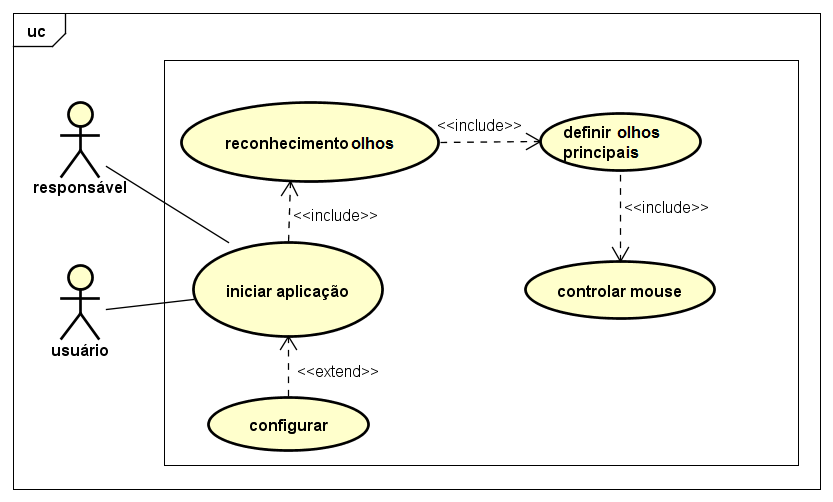
\includegraphics[scale=.5]{img/UseCase_Diagram_2.png}

{\fontsize{11}{11}\selectfont \textbf{Fonte:} Elaborada pelo autor.}
\label{fig:use-case-diagram}
\end{figure}

O início do funcionamento é marcado pela inicialização da aplicação, representado como a elipse “Iniciar aplicação” no diagrama. Em seguida é feito o reconhecimento dos olhos, representado pela elipse “Reconhecer olhos” no diagrama, a aplicação ainda define qual das duplas de olhos ele deve rastrear, esta funcionalidade é representada pela elipse “Definir olhos principais” no diagrama.  Após isto é dado o controle do \textit{mouse} para o usuário, é feita uma simulação do \textit{mouse}, representado pela elipse “Controlar mouse”, além disto é possível entrar na área de configuração a qualquer momento, representado pela elipse “Configurar”.

% \subsection{Diagrama de Classes}
% O Diagrama de Classes é o mais utilizado e o mais importante da UML. É extremamente relevante junto com o paradigma de Orientação a Objetos. E serve de apoio para a maioria dos demais diagramas. Como o próprio nome diz, define a estrutura das classes utilizadas pelo sistema, determinando os atributos e métodos que cada classe possui, segundo \citeonline{guedes2011uml}. O Diagrama da Figura \ref{fig:diagrama-classes} apresenta o diagrama utilizado para modelagem do VisiUMouse, a classe “Detector” tem grande destaque, é ela que detecta e rastreia os olhos do usuário, ela está representada no diagrama como “Detector”. Outra classe importante é a responsável por simular o \textit{mouse}, dando o controle do computador para o usuário, está representado como “Mouse” no diagrama. E por fim a classe “Main” que é a responsável por controlar as outras classes. 

% \begin{figure}[htbp]
% \caption{Diagrama de Classes.} 
% \centering 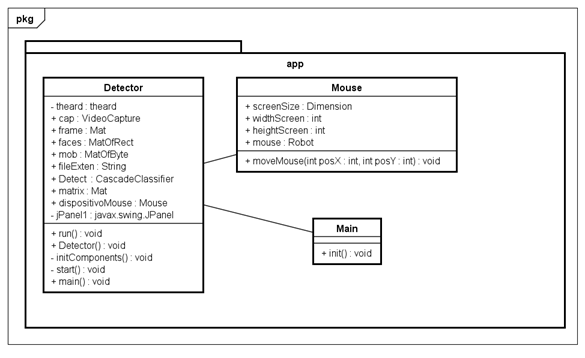
\includegraphics[scale=1]{img/diagrama-classes.png}
% \textbf{Fonte:} Autor.
% \label{fig:diagrama-classes}
% \end{figure}


% \subsection{Diagrama de Sequência}
% O Diagrama de Sequência apresenta a ordem temporal em que as mensagens são trocadas entre os objetos envolvidos em uma determinada função. Em geral, baseia-se em um Caso de Uso definido pelo diagrama de mesmo nome e tem como base o Diagrama de Classes para determinar os objetos das classes envolvidas em um processo, segundo \citeonline{guedes2011uml}. A Figura \ref{fig:diagrama-sequencia} apresenta o Diagrama de Sequência do VisiUMouse.

% O início da representação temporal do diagrama é dada pela ação do Ator “Usuário”, no momento que ele iniciar a aplicação “1.1 init app()”, o qual vai começar a detectar os olhos na entrada de vídeo, ou seja no momento que o programa foi executado e a entrada de vídeo (\textit{webcam}) estiver fornecendo dados a aplicação vai detectar todos os olhos presentes no vídeo. Quando a aplicação identifica mais de uma dupla de olhos é determina qual dupla deve ser rastrear e usada para controlar o computador, esta funcionalidade está representada no diagrama como “3.1 Detectar Olhos”. E na etapa final é dado o controle do computador para o usuário através da simulação das funcionalidades do \textit{mouse}, no diagrama está representado como “”3.2 Controlar mouse()”. 

% \begin{figure}[htbp]
% \caption{Diagrama de Sequencia.}
% \centering 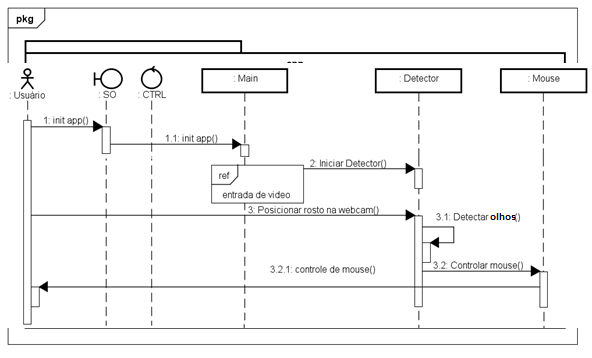
\includegraphics[scale=1]{img/diagrama-sequencia.png}
% \textbf{Fonte:} Autor.
% \label{fig:diagrama-sequencia}
% \end{figure}

\chapter{DESIGN}\label{CAP6}
A importância do Design está no desenvolvimento de produtos (digitais ou físicos) que facilitem a vida das pessoas ele possibilita criar coisas funcionais e bonitas. O Design pode dar destaque a um produto com as mesmas funcionalidade e preço de outros. Por isso o Design é o fator decisivo no sucesso ou fracasso de um produto. Assim como um Design bem pensado desperta o desejo dos consumidores, um Design pobre e mal feito gera uma repulsa enorme, segundo \citeonline{patterson2017computer}.

Este trabalho apresenta o Design do \textit{software} e site do VisiUMouse, o \textit{software} é uma tecnologia \textit{desktop} que é executado pelo usuário na área de trabalho do computador, permitindo que ele controle o computador; o site é o responsável por apresentar e disponibilizar o VisiUMouse na \textit{Web} para os usuários, entre outras funcionalidades.

\section{DESIGN DO SOFTWARE DESKTOP}\label{Sub:software}
Para a criação da interface foram utilizados os conceitos de CRAP (Contraste, Repetição, Alinhamento e Proximidade) apresentados na disciplina de Design de Interface, a escolha da paleta de cores foram definidas através de um levantamento das principais cores das tecnologias Digitais atuais, foi feito uma pequena alteração nesta paleta para torná-la única e por consequência uma característica da própria tecnologia, as outras estilizações como sombra e tipografia foram definidas através das tendências atuais. Além de seguir boas práticas de \textit{Graphical User Interface} (GUI) para pessoas com pouca mobilidade, por exemplo botões grandes e mais afastados. A Figura \ref{fig:interface-tecnologia} mostra a tela principal do \textit{software} VisiUMouse.

\begin{figure}[htbp]
\caption{Interface principal do VisiUMouse.} 
\centering 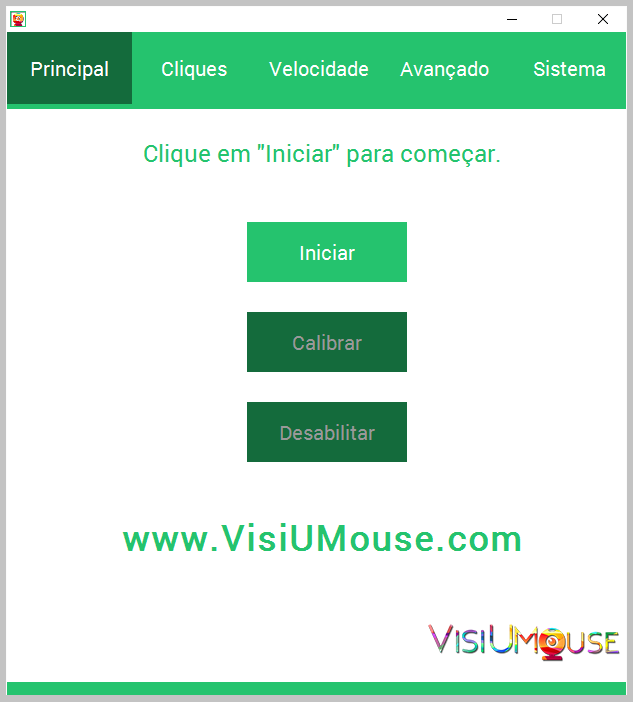
\includegraphics[scale=.5]{img/visiumouse-tela-principal-v216.png}

{\fontsize{11}{11}\selectfont \textbf{Fonte:} Elaborada pelo autor.}
\label{fig:interface-tecnologia}
\end{figure}

\section{DESIGN DO SITE}\label{Sub:site}

O desenvolvimento do site tem como objetivo disponibilizar todo o conteúdo referente ao VisiUMouse, como o próprio \textit{software}, informações, módulos que foram criados juntamento com o VisiUMouse, uma página de contato entre outros. A Figura \ref{fig:site} apresenta a página inicial do site, no topo esta presente o menu de navegação que é fixo que permite que o usuário navegue entre todo o site de forma simples.

\begin{enumerate}
\item \textbf{inicial}: esta representado como a logo do site, do lado extremo esquerdo, ao clicar nessa imagem o usuário volta para o inicio da página.
\item \textbf{videos}: essa seção mostra um conjunto de vídeos que tem como objetivo dar uma visão geral do VisiUMouse
\item \textbf{funcionamento}: apresenta uma explicação resumida de como utilizar o VisiUMouse.
\item \textbf{contato}: nessa seção é possível enviar uma mensagem para o site.
\end{enumerate}


\begin{figure}[htbp]
\caption{Interface da página inicial do Site.} 
\centering 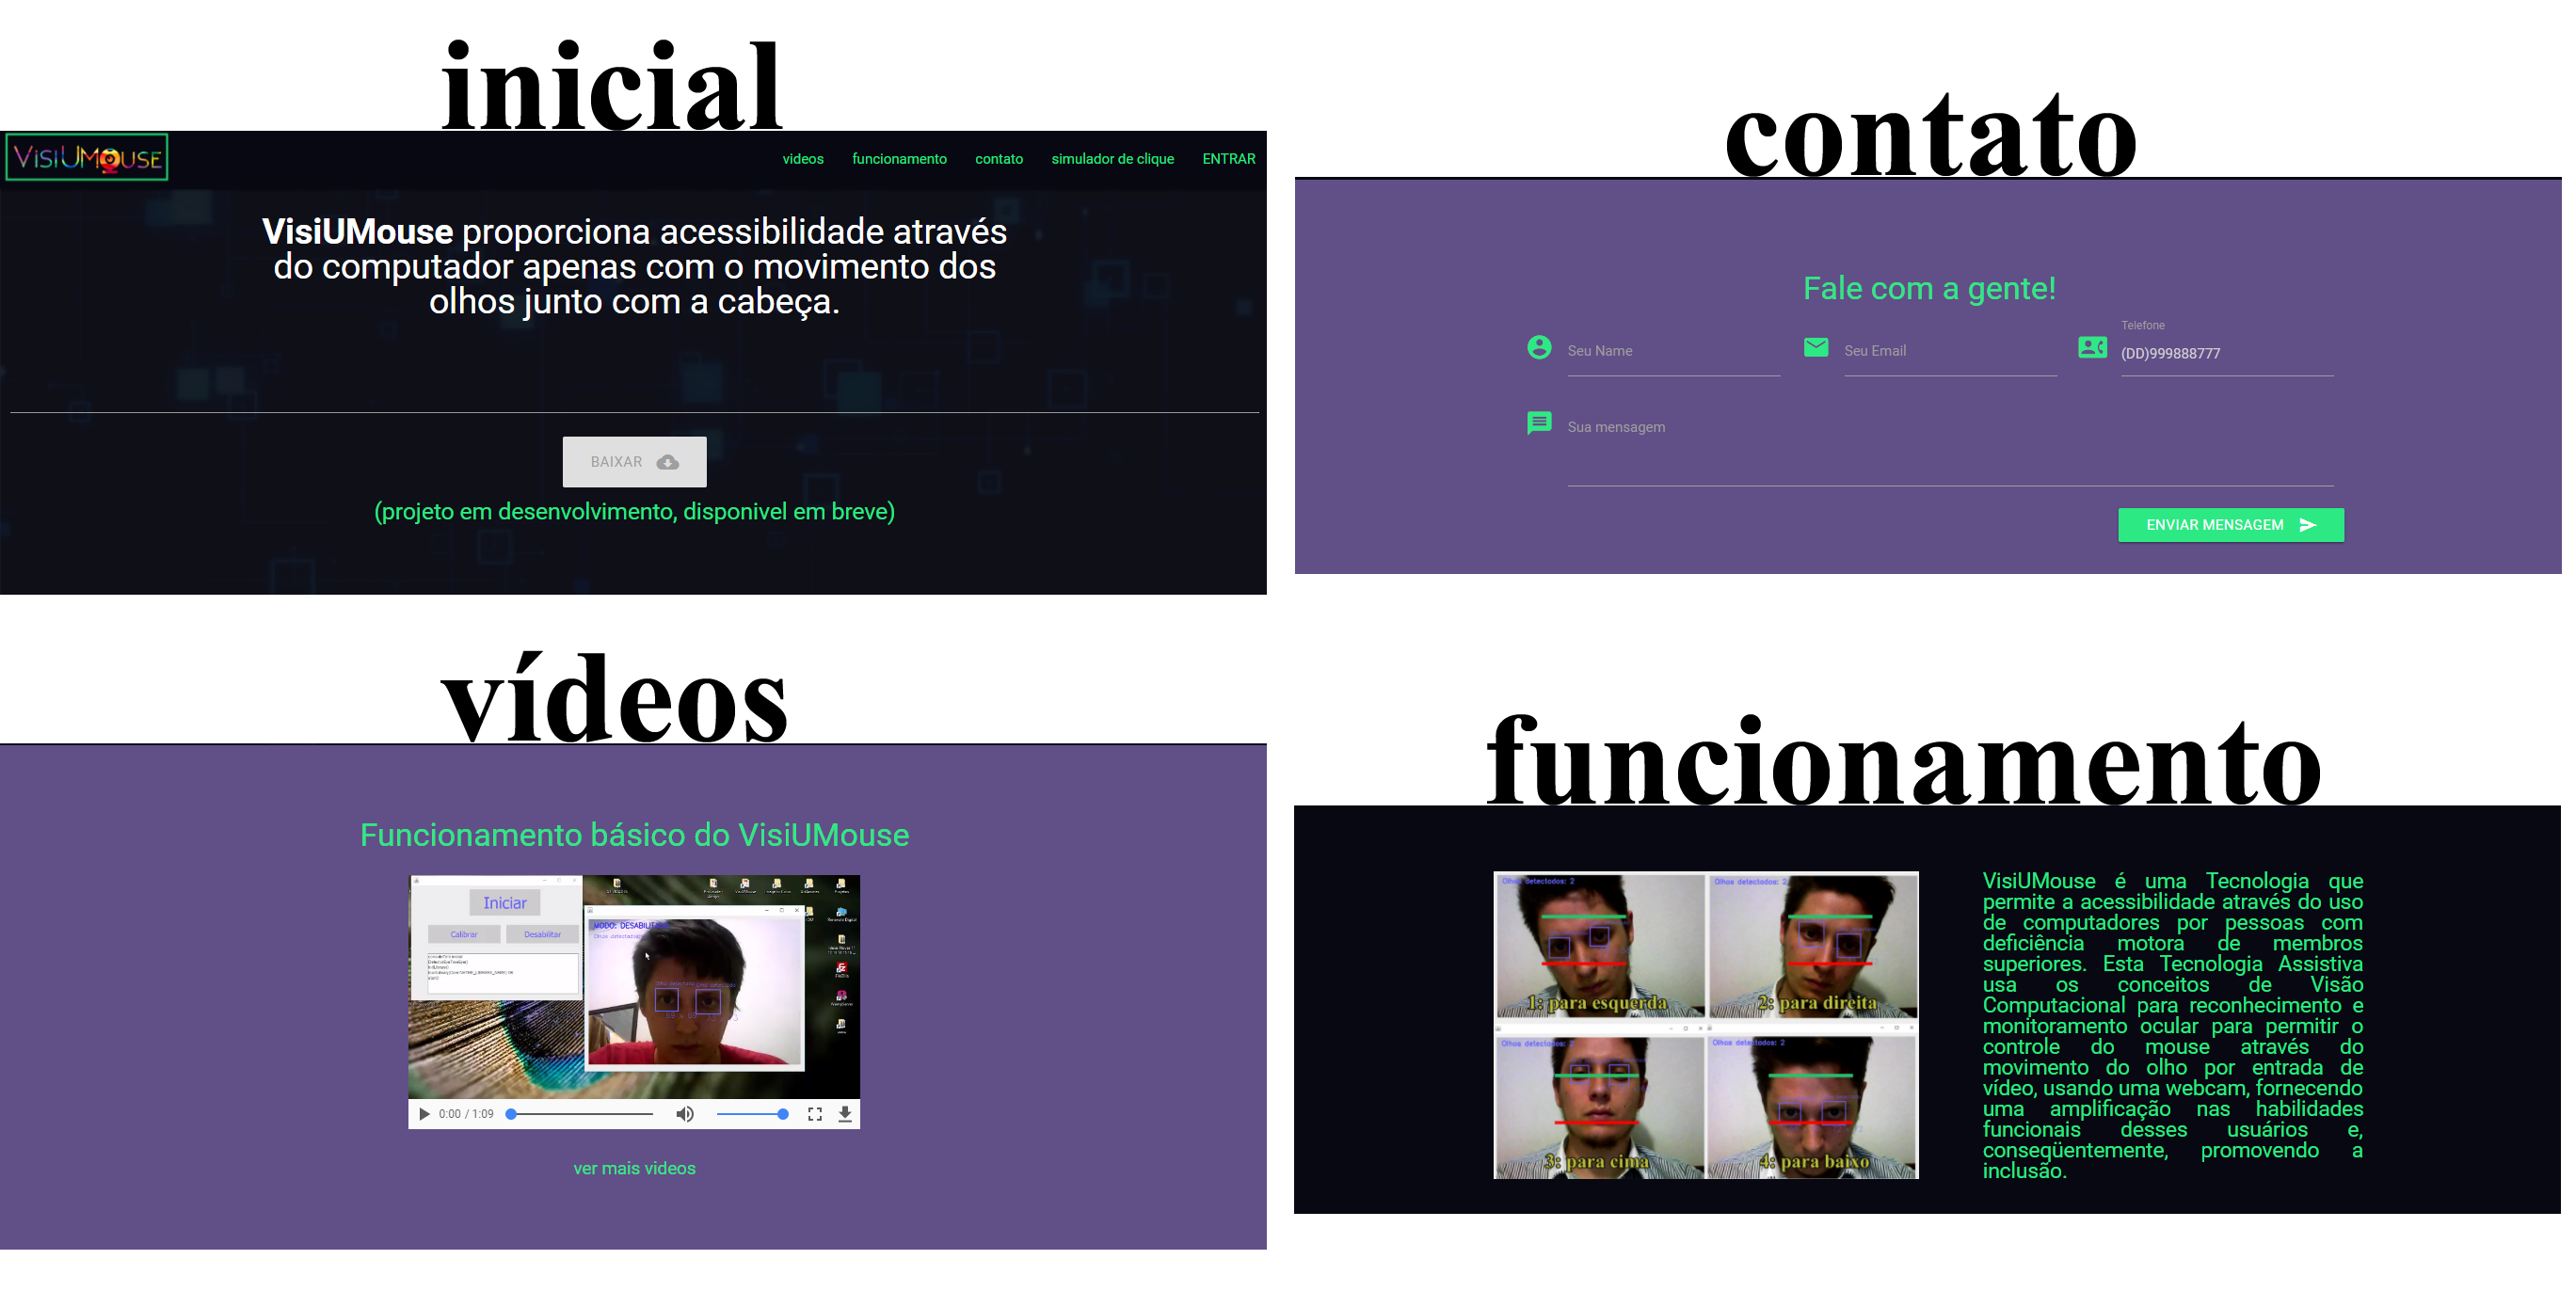
\includegraphics[scale=.33]{img/site.png}

{\fontsize{11}{11}\selectfont \textbf{Fonte:} Elaborada pelo autor.}
\label{fig:site}
\end{figure}

\chapter{TECNOLOGIAS UTILIZADAS}\label{CAP6-tecnilogias-utilizadas}
Esse Capítulo apresentam o conjunto de tecnologias utilizadas e desenvolvidas nesse trabalho, por questão de organização será segmentando 2 partes, as tecnologias utilizadas no site e no software.

\section{Software Desktop}\label{Sub:tecnologias-software}
Essa sessão aponta as principais tecnologias utilizadas para o desenvolvimento da aplicação \textit{desktop}, ou seja o software que será executado pelo usuário no seu computador. A principal tecnologia utilizada foi a Linguagem de Programação Java, entre suas características podemos citar possibilidade de desenvolver em multiplataforma, isso permite que um mesmo \textit{software} seja executado em diferentes Sistemas Operacionais, como Linux, Windows, Android, entre outros. Além de Java foi utilizado a Linguagem de Programação C a biblioteca OpenCV e o \textit{software} Install Creator. 

Para o desenvolvimento do \textit{software} VisiUMouse foi criado um conjunto de ferramentas para auxiliar, como um Simulador de \textit{Mouse}; um \textit{script} para otimizar o controle de versões, o Auto Commit e um protocolo para metrificar testes, o Fitts Task Two, os quais estão presentes nos tópicos seguintes.

\begin{enumerate}
\item \textbf{Java}

Criada pela equipe de desenvolvedores liderada por James Gosling na Sun Microsystems (atualmente de propriedade da Oracle) e lançada em 1995, o Java é uma linguagem de programação Orientada a Objetos que atualmente faz parte do núcleo da Plataforma Java. A Orientação a Objetos, ou Programação Orientada a Objetos (POO), é um tipo de paradigma de análise, para a programação de sistemas no qual todos os elementos inseridos são objetos. \cite{urma2014java}.

A linguagem Java possui arquitetura neutra e portável, de forma que pude ser utilizada em diversos Sistemas operacionais, ter alta performance, apresentar segurança e solidez e ser uma linguagem interpretada com suporte a \textit{threads} e dinâmica. As aplicações em Java normalmente podem ser executadas em qualquer plataforma que possua a Java Virtual Machine (JVM) instalada, independente da arquitetura do computador.

O Java utiliza o \textit{Garbage Collector} para gerenciar a memória referente ao ciclo de vida dos objetos e sua permanência nela. O programador determina quando os objetos são criados e o Java \textit{Runtime} é responsável pela retirada do objeto da memória quando ele não estiver mais em uso, evitando que este processo seja feito manualmente como nas linguagens de programação estruturada.


\item \textbf{Linguagem C}

A linguagem C foi criada por Dennis Ritchie em 1972 com um propósito: ser usada no desenvolvimento de uma nova versão do sistema operacional Unix. A primeira versão do Unix utilizava Assembly. Além de toda essa flexibilidade, C é capaz de gerar programas extremamente rápidos em tempo de execução, possui uma sintaxe simples e poderosa, com instruções de alto nível. A linguagem C influenciou de forma direta muitas linguagens como C++, Java, C\# , Objective C, e muitas outras linguagens de programação tem sua sintaxe e estruturas influenciadas por C, segundo \citeonline{backes2012linguagem}.

Entre suas características principais podem citar: a Portabilidade, geração de códigos executáveis compactos e rápidos, interação com o Sistema Operacional e linguagem estruturada. A geração de códigos compactos e rápido ganha destaque nos algoritmos de PDI, que demandam processar uma grande quantidade de dados, os quais representam a leitura e reconhecimento de padrões dos \textit{pixels} de uma imagem.

\item \textbf{OpenCV}

O OpenCV (\textit{Open Source Computer Vision Library}) é uma biblioteca multiplataforma desenvolvida pela Intel Corporation, que implementa diversos módulos para VC, este os quais são utilizados para o Processamento de Imagens e Vídeo, Estruturas de dados, álgebra linear e mais de 350 algoritmos de VC. OpenCV possui, em seu módulo central uma implementação do algoritmo de Viola-Jones para detecção de objetos, de acordo com \cite{bradski2008learning}.

\item \textbf{Simulador de Mouse}

O Simulador\footnote{O Simulador está disponível em: https://github.com/KrishnaXavier/system-click-time} é uma aplicação capaz de simular um \textit{mouse} comum, com o clique com base no tempo, isto é o clique é gerado após um determinado tempo parado, esse tempo pode ser configurado, além disso ele também simula os principais cliques de um \textit{mouse}, como o clique do botão primário (geralmente é representado pelo botão esquerdo do \textit{mouse}), duplo primário, botão secundário (geralmente é representado pelo botão direito do \textit{mouse}) e a função de arrastar. Ele possibilita manter as métricas do \textit{clique} igual para testes comparativos entre diferentes dispositivos, como o experimento descrito no Capítulo \ref{CAP7}, que apresenta um teste de comparação do VisiUMouse com o \textit{mouse} tradicional.

\item \textbf{Fitts Task Two}

O Fitts Task Two\footnote{O Protocolo está disponível em: https://github.com/KrishnaXavier/FittsTaskTwo} é um protocolo baseado na Lei de Fitts, proposto por \citeonline{soukoreff2004towards}, ele permite metrificar o ato de "apontar" na movimentação humana, como o controle \textit{mouse}. Ele foi criado a partir de um outro \textit{software} de código aberto disponível na \textit{internet}, boa parte do código foi mantida, foram feitas apenas altercações necessárias para realizar o experimento descrito no Capítulo \ref{CAP7}.

\item \textbf{Auto Commit}

O Auto Commit\footnote{O Auto Commit está disponível em: https://github.com/KrishnaXavier/auto-commit} é uma sequência de comandos implementados em um \textit{software} executável, ou seja, um \textit{script}, que permite salvar as alterações de qualquer aplicação de forma mais amigável, apenas com um comando. Esse \textit{script} foi criando visando ajudar os desenvolvedores e colegas que tinham dificuldade em salvar as alterações das suas aplicações.

\end{enumerate}

\section{Site}\label{Sub:tecnologias-site}
As tecnologias utilizados no desenvolvimento do site foram divididas em 2 categorias, as que funcionam no lado do servidor (\textit{Server-side}) e as que funcionam apenas no lado do cliente e do navegador (\textit{Client-side}). Entre as tecnologias \textit{Server-side} podemos citar o PHP e MySQL. E entre as tecnologias \textit{Client-side} podemos citar HTML5, CSS, JavaScript, \textit{Framework }JQuery e \textit{Framework} Materialize. Além disso foram utilizadas as arquiteturas MVC e SPA. Para a criação da estrutura do PHP Orientado a Objetos foi desenvolvido uma ferramenta facilitar, o Creator OOP Structure.

\begin{enumerate}
\item \textbf{PHP 5}

A linguagem de programação PHP (um acrônimo recursivo para PHP: Hypertext Preprocessor) é uma linguagem de \textit{script} de código aberto de uso geral, muito utilizada, e especialmente adequada para o desenvolvimento web e que pode ser embutida dentro do HTML. Ela frequentemente é utilizada para a comunicação com o Banco de Dados. A linguagem permite que se adicione dinamicidade aos projetos web, ou seja, o conteúdo da página é montado durante a requisição e então enviado ao cliente, segundo \citeonline{converse2003php}.

\item \textbf{MySQL}

O sistema MySQL foi desenvolvido pela empresa sueca MySQL AB e publicado, originalmente, em maio de 1995. O MySQL é um sistema de gerenciamento de banco de dados (SGBD) de código aberto, que utiliza a linguagem SQL (Linguagem de Consulta Estruturada, do inglês \textit{Structured Query Language}) como interface. É atualmente um dos sistemas de gerenciamento de Bancos de Dados mais populares, com mais de 10 milhões de instalações pelo mundo, de acordo com \cite{miletto2014desenvolvimento}.

\item \textbf{HTML5}

Como \citeonline{silva2015fundamentos} define, o HTML (abreviação para a expressão inglesa \textit{HyperText Markup Language}, que significa Linguagem de Marcação de Hipertexto) é uma linguagem de marcação utilizada na construção de páginas na Web. Documentos HTML podem ser interpretados por navegadores. A tecnologia é fruto da junção entre os padrões HyTime e SGML. Atualmente sua versão é a 5.0.

\item \textbf{CSS3}

CSS3 é a segunda mais nova versão das famosas \textit{Cascading Style Sheets} (ou simplesmente CSS), onde se define estilos para páginas web com efeitos de transição, imagem, e outros, que dão um estilo novo às páginas Web em todos os aspectos de design do layout. CSS3 ultrapassou o status de proposta de uma tecnologia que prometia revolucionar a forma como estilizamos documentos para a web e deve obrigatoriamente fazer parte do dia a dia dos designers e desenvolvedores web, segundo \citeonline{silva2011css3}.

\item \textbf{JavaScript}

JavaScript é uma linguagem de programação interpretada que foi originalmente implementada como parte dos navegadores Web para que \textit{scripts} pudessem ser executados do lado do cliente e interagissem com o usuário sem a necessidade deste \textit{script} passar pelo \textit{Server-side}, controlando o navegador, realizando comunicação assíncrona e alterando o conteúdo do documento exibido. \cite{flanagan2007javascript-UPPERCASE}.

\item \textbf{Framework Materialize}

Materialize é um \textit{framework} \textit{Client-side} que resolve os mesmos problemas como alinhamento de objetos HTML e Desgin Responsivo. Ele surgiu através de um projeto desenvolvido pela Google e é inspirado no Material Design (design utilizado no sistema operacional para \textit{smartphones} Android desde a versão 5.0).

\item \textbf{Framework {j}Query}

O \textit{Framework} jQuery em JavaScript permite a abstração de tarefas comuns do \textit{Client-side}, como a manipulação de elementos da página, gerenciamento de eventos, requisições e Ajax. O jQuery permitiu uma codificação rápida e direta, diminuindo o código e o tornando mais legível, o que consequentemente tornou o desenvolvimento mais eficiente, \cite{duckett2018javascript}. Com o Ajax é possível implementar a arquitetura SPA, que esta descrita no tópico seguinte.

\item \textbf{Arquitetura SPA}

Um aplicativo de página única (\textit{Single Page Application}, ou SPA) é uma aplicação web ou site que consiste de uma única página web com o objetivo de fornecer uma experiência do usuário similar à de um aplicativo desktop. Em um SPA, todo o código necessário - HTML, JavaScript, e CSS – ou é obtido com um único carregamento de página, ou os recursos apropriados são carregados dinamicamente e adicionados à página conforme necessário, geralmente em resposta a ações do usuário. A página não é recarregada em qualquer momento do processo, tampouco ocorre a transferência de controle para outra página. Interação com aplicativos de página única muitas vezes envolve comunicação dinâmica com o servidor web por trás dos bastidores, de acordo com \citeonline{mikowski2013single}.

\item \textbf{Arquitetura MVC}

Segundo \citeonline{teruel2012arquitetura} a arquitetura MVC é padrão de \textit{software} que permite dividir a aplicação em 3 camadas, \textit{Model}, \textit{View} e \textit{Controller}. O \textit{Model} consiste nos dados da aplicação, regras de negócios, lógica e funções. Uma \textit{View} pode ser qualquer saída de representação dos dados, como uma tabela ou um diagrama. É possível ter várias visões do mesmo dado, como um gráfico de barras para gerenciamento e uma visão tabular para contadores. O \textit{Controller} faz a mediação da entrada, convertendo-a em comandos para o \textit{Model} ou \textit{View}. As ideias centrais por trás do MVC são a reusabilidade de código e separação de conceitos.

\item \textbf{Creator OOP Structure}

Creator OOP Structure\footnote{O Creator OOP Structure está disponível em: https://github.com/KrishnaXavier/creator-oop-structure}  é uma ferramenta que auxilia a criação da estrutura do PHP Orientado a Objetos de forma a deixar a codificação mais rápida, para criar toda a estrutura ele apenas precisa do nome da classe, os seus atributos e as respectivas visibilidades.

\end{enumerate}


\chapter{TUTORIAL DO VISIUMOUSE}\label{CAP-tecnologia-visiumouse}
Neste Capítulo é manifestado a visão do usuário final, desde o cadastro e entrada no site para fazer o \textit{download}, até a instalação e uso do VisiUMouse. 

\section{Download do VisiUMouse}
Para qualquer usuário que deseja fazer o \textit{download} do VisiUMouse é obrigatório o cadastro, caso não tenha se cadastrado antes, caso já tenha se cadastrado em um outro momento é preciso apenas efetuar a entrada (\textit{login}), para isso foi criado uma sessão no menu que corresponde a essas funcionalidades, a "ENTRAR", na Figura \ref{fig:site-entrar} podemos ver essa opção no canto superior direito, marcado com vermelho. Ao clicar nessa opção o usuário vai entrar na página entrar, como mostrado em "Página de entrada", a qual ele pode inserir seus dados para entrar no site, porém caso ele não tenha se cadastrado ele pode clicar em "CADASTRAR", ainda na mesma página, após clicar em "CADASTRAR" é carregado a página de cadastro, como mostrado na Figura \ref{fig:site-entrar} na "Página de cadastro". Para fazer o cadastro é necessário o usuário informar seus dados pessoais, se alguma informação estiver incorreta o próprio site vai indicar. 

\begin{figure}[H]
\caption{Páginas de cadastro e entrada de usuários do site.} 
\centering 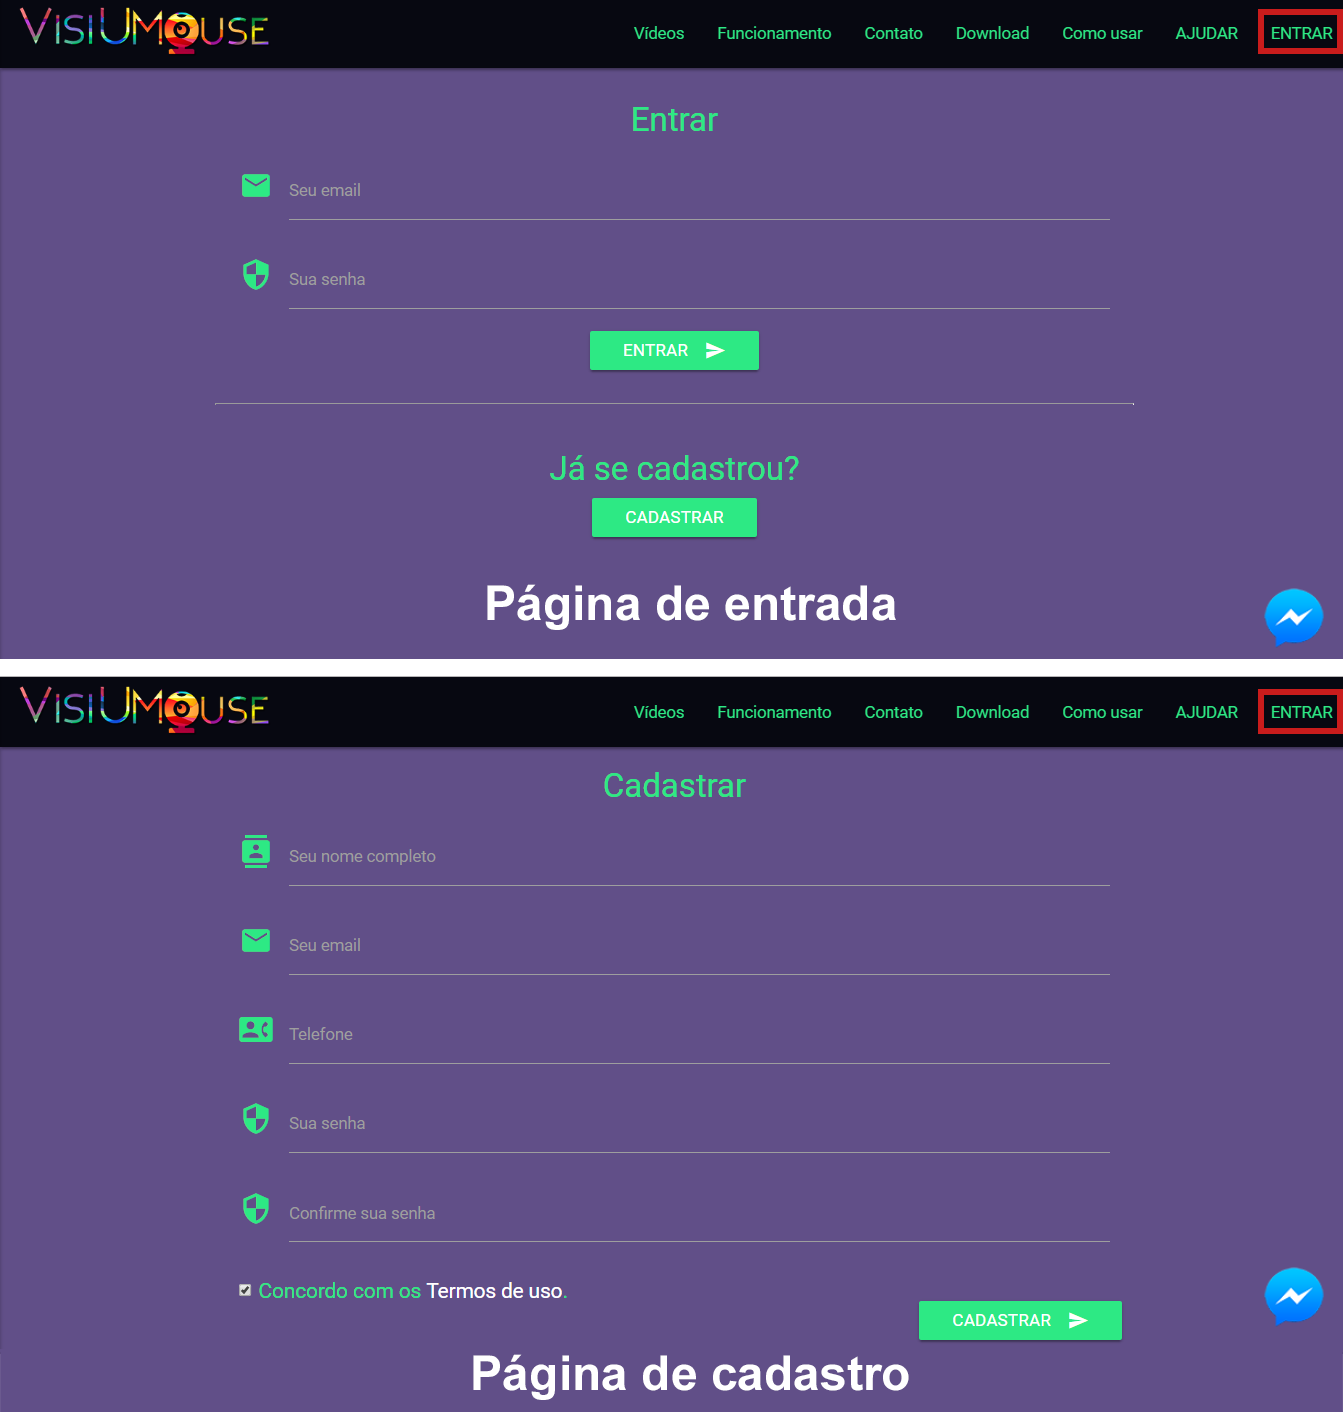
\includegraphics[scale=0.45]{img/site-entrar.png}

{\fontsize{11}{11}\selectfont \textbf{Fonte:} Elaborada pelo autor.}
\label{fig:site-entrar}
\end{figure}

Após a entrada do usuário no site é possível fazer o \textit{download} do VisiUMouse, nessa página ele pode ver um tabela com características de cada versão, como mostrado na Figura \ref{fig:site-download}.

\begin{figure}[H]
\caption{Página de downloads do site.} 
\centering 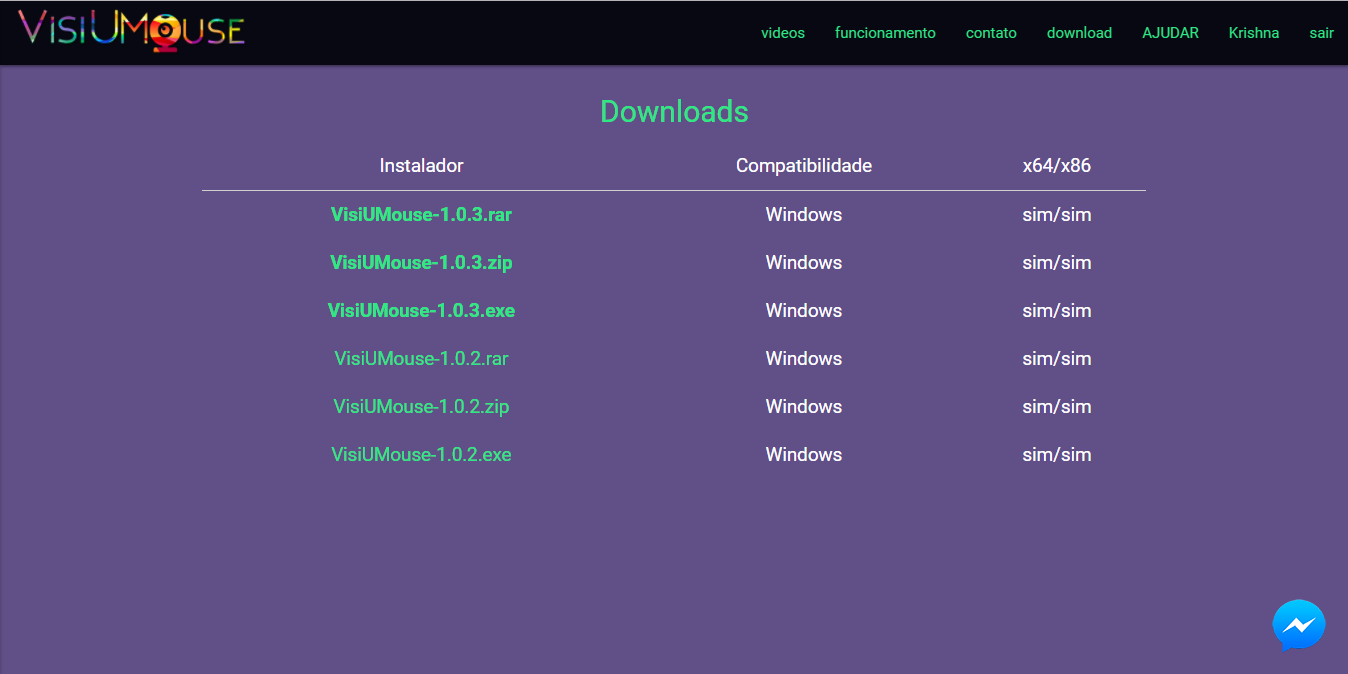
\includegraphics[scale=0.35]{img/site-download.png}

{\fontsize{11}{11}\selectfont \textbf{Fonte:} Elaborada pelo autor.}
\label{fig:site-download}
\end{figure}

\section{Instalando o VisiUMouse}
A instalação do VisiUMouse segue o padrão de outros instaladores de \textit{softwares} disponíveis no mercado, a primeira tela é de apresentação, explicando o que o instalador vai fazer e se o usuário concorda; uma tela onde é configurado a pasta onde o VisiUMouse vai ser instalado; uma tela para iniciar a instalação; e, por fim, uma tela avisando que o VisiUMouse já foi instalado, como mostrado na Figura \ref{fig:visiumouse-instalador}.

\begin{figure}[H]
\caption{Telas de instalação do VisiUMouse.} 
\centering 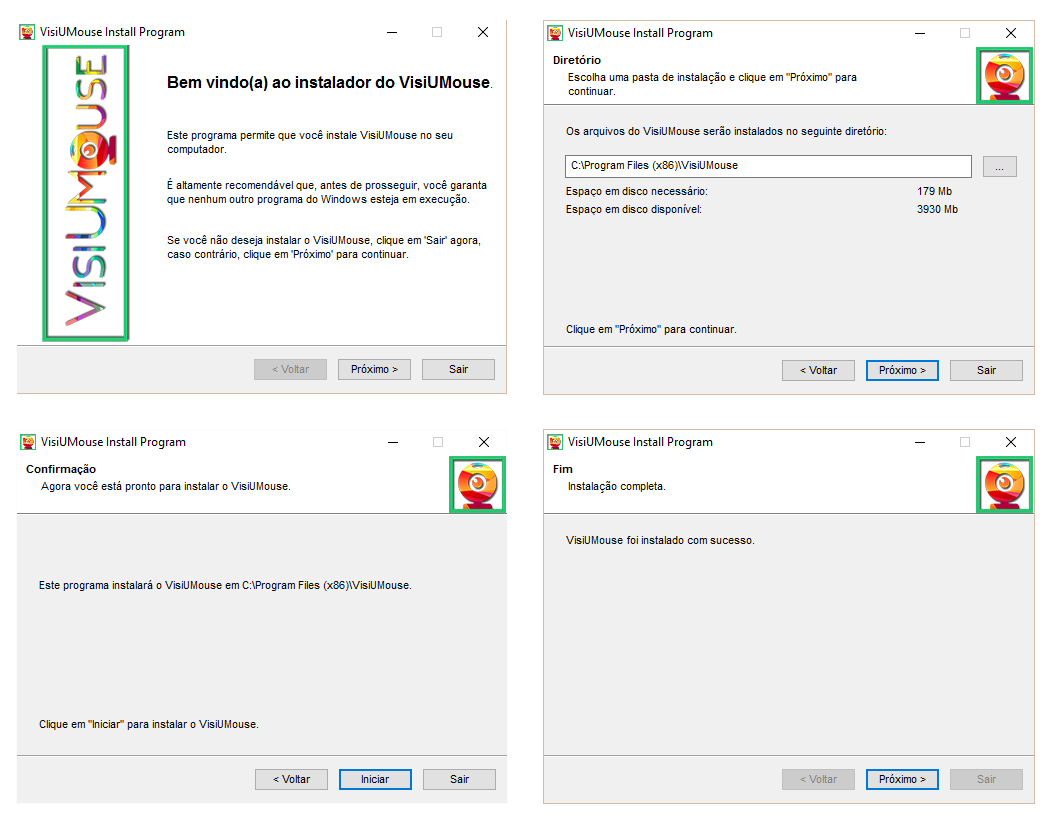
\includegraphics[scale=0.45]{img/software-instalador.png}

{\fontsize{11}{11}\selectfont \textbf{Fonte:} Elaborada pelo autor.}
\label{fig:visiumouse-instalador}
\end{figure}

\section{VisiUMouse}
Após a instalação, o VisiUMouse pode ser executado através de um atalho que foi criado na área de trabalho. A primeira tela que renderizada é a tela principal da GUI, como vista na Figura \ref{fig:visiumouse-tela-principal}, é ela que tem os primeiros passos para iniciar o controle do movimento e clique do \textit{mouse}. No primeiro momento é preciso clicar no botão "iniciar", para iniciar a \textit{webcam}.

\begin{figure}[H]
\caption{Tela principal do VisiUMouse.} 
\centering 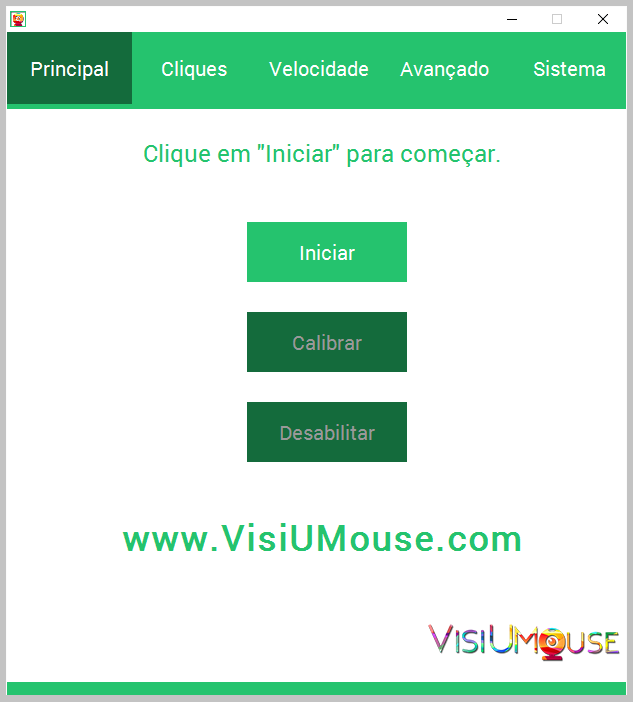
\includegraphics[scale=.5]{img/visiumouse-tela-principal-v216.png}

\textbf{Fonte:} Elaborada pelo autor.
\label{fig:visiumouse-tela-principal}
\end{figure}

A inicialização da \textit{webcam} é dada pela tela de captura de vídeo, como visto na Figura \ref{fig:visiumouse-tela-captura-video}, ela permite que e o usuário tenha o retorno se ele esta posicionado no centro da tela, e se é possível rastrear seus olhos, os retângulos vermelho em volta dos olhos mostram o rastreamento dos olhos. Nessa tela o usuário pode ver o "MODO" da aplicação, como visto no canto superior esquerdo da Figura, podendo dar 3 avisos: "FUNCIONAL" mostrando que já é possível controlar o movimento do \textit{mouse}; "DESABILITADO" informa o usuário que ele não está controlando o \textit{mouse}; "CALIBRANDO (FIQUE PARADO(A))" que informa o usuário que não deve se mover por que o VisiUMouse esta calibrando.

No segundo momento é preciso clicar em "calibrar" para calibrar o VisiUMouse, ou seja o usuário precisa ficar parado até receber o aviso que o modo está funcional, como visto na Figura \ref{fig:visiumouse-tela-captura-video}. Após a calibração o usuário é capaz de controlar o \textit{mouse} e para desabilitar o controle basta clicar em "desabilitar" na tela principal, como visto na Figura \ref{fig:visiumouse-tela-principal}.

\begin{figure}[H]
\caption{Tela de captura de vídeo.} 
\centering 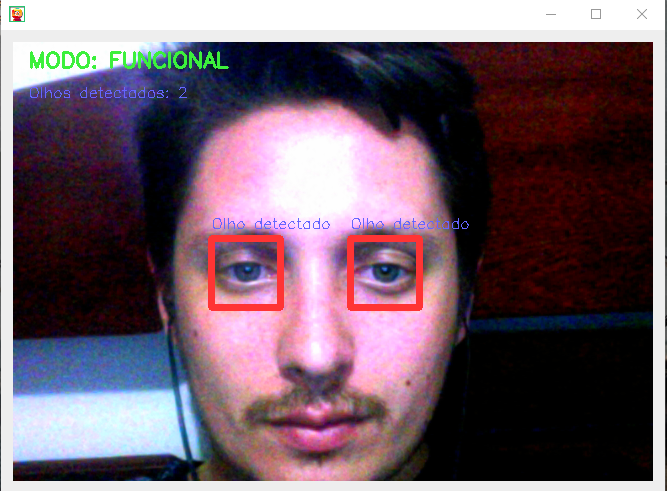
\includegraphics[scale=.45]{img/visiumouse-tela-captura-video.png}

{\fontsize{11}{11}\selectfont \textbf{Fonte:} Elaborada pelo autor.}
\label{fig:visiumouse-tela-captura-video}
\end{figure}

\chapter{EXPERIMENTO}\label{CAP7}

% Dissertação do vinicius: https://www.overleaf.com/read/gbykffbhwqtk#/42933380/
% Capitulo 4 fala sobre os testes

O experimento foi executado por 9 participantes voluntários, com idade média de 23,3 anos, com o objetivo de fazer uma avaliação comparativa do \textit{software} VisiUMouse com o \textit{mouse} convencional para avaliar o seu funcionamento e objetivo. Para tanto foi utilizado um protocolo baseado na lei de Fitts, proposto por \citeonline{soukoreff2004towards}, envolvendo tarefas comuns como apontar, selecionar e clicar, que são usadas como métricas para verificar a interação com o computador. O protocolo foi configurado para 6 etapas, com 5 alvos cada, podendo ter o tamanho de 120, 150 ou 180 pixeis. O tamanho (gerados aleatoriamente) de cada um dos 5 alvos são iguais para cada fase \footnote{Foi disponibilizado gravações dos testes em: http://visiumouse.com}.

O teste foi dividido em 3 etapas: a primeira consistiu na aprendizagem de uso da aplicação, onde o participante era familiarizado com o funcionamento do VisiUMouse durante 5 minutos; a segunda etapa consistiu no experimento em si com o VisiUMouse; na última etapa, o participante utilizou o \textit{mouse} convencional para a execução das mesmas tarefas da etapa anterior. Os resultados são computados pelo \textit{software} do protocolo.

Para as três etapas foi utilizado o clique por tempo, denominado \textit{dwell time}, segundo \citeonline{gips2000camera}, configurado para o tempo 5 segundos para efetuar o clique. Cabe ressaltar que em paralelo ao desenvolvimento do VisiUMouse foi criado um \textit{software} de clique por tempo para ser usado nos testes \footnote{Software de clique por tempo. Disponível em: http://visiumouse.com}. As demais configurações do VisiUMouse como velocidade foram mantidas iguais em todos os testes.  

O experimento foi conduzido com um notebook (LG S460) equipado com Windows 10, processador 2,4GHz (i3), 4 GB RAM, monitor de 14 polegadas, resolução de 1366 x 768 pixeis e utilizou-se a \textit{webcam} do próprio computador.

O interesse do Experimento é em nível de protótipo, para tentar garantir que o desenvolvimento está no caminho certo, e para avaliar se o produto final atende ao público-alvo, porém quando se trata de pessoas com deficiência motora, no primeiro momento é necessário uma rodada de testes com pessoas sem nenhuma deficiência, conforme \cite{stone2005user}, para que os testes com o público-alvo já estejam cuidadosamente planejados e refinados. Além de buscar, com os profissionais da área de Terapia Ocupacional, conforme \cite{oliveira2015uso}, aspectos multidisciplinares relacionados a prescrição, habilidades e necessidades dos usuários.

\section{RESULTADOS}\label{Sub:resultados-ex-1}
A Figura \ref{fig:assertividade} apresenta o gráfico dos resultados da assertividade dos cliques nos alvos. O software VisiUMouse (VUM, em azul) teve assertividade média de 99,63\%, representando apenas um erro com o participante 8. O \textit{mouse} comum (Mouse, em laranja) teve assertividade de 100\%, que já era esperado devido a grande familiaridade que os usuários já tinham com este dispositivo.

\begin{figure}[htbp]
\caption{Resultados da assertividade dos cliques nos alvos.} 
\centering 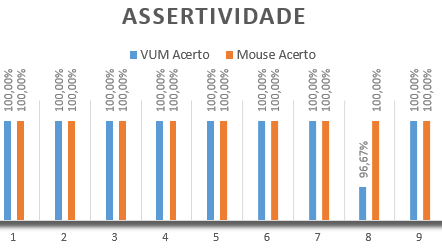
\includegraphics[scale=1]{img/assertividade.png}

{\fontsize{11}{11}\selectfont \textbf{Fonte:} Elaborada pelo autor.}
\label{fig:assertividade}
\end{figure}

A Figura \ref{fig:tmc} apresenta o gráfico com os resultados do tempo médio de cada clique (TMC), em milissegundos. O TMC do \textit{mouse} comum foi de aproximadamente 6372,4 milissegundos. O VisiUMouse (VUM) teve o TMC de aproximadamente 16579,5 milissegundos.
\begin{figure}[htbp]
\caption{Resultados do teste comparativo.} 
\centering 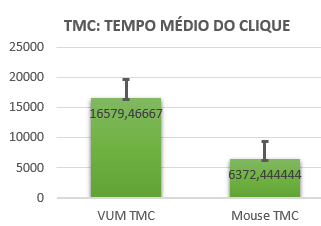
\includegraphics[scale=1.5]{img/tmc2.png}

{\fontsize{11}{11}\selectfont \textbf{Fonte:} Elaborada pelo autor.}
\label{fig:tmc}
\end{figure}

\chapter{CONSIDERAÇÕES FINAIS E TRABALHOS FUTUROS}\label{CAP-consideracoes-finais-trabalhos-futuros}

A solução proposta, o VisiUMouse, está disponível para qualquer pessoa que tenha acesso a \textit{internet}, no site "www.VisiUMouse.com", para qualquer tipo de usuário ou estudo, entre outras aplicações. Apesar de já ter lançado uma versão final (alpha) ainda podem ser desenvolvidas outras versões, de acordo com a necessidade dos usuários.

Entre os desafios enfrentados se destacou o estudo e implementação relacionados as áreas de VC, \textit{Machine Learning} e aplicações \textit{desktop}. Esses desafios foram ultrapassados com uma grande força de vontade e ambição de fazer algo diferente.

Esse trabalho só foi possível por causa te todas as pessoas envolvidas, como orientadores e professores; experiências adquiridas em grupos de pesquisa como WeTech e IOM; e os conhecimentos adquiridos no curso, os quais estão presente nesse trabalho.

Entre os trabalhos futuros estão a implementação do rastreamento da visão, para os usuários que não tem a movimentação da cabeça; a implementação de uma aplicação para dispositivos móveis (celulares e \textit{tablets}) com as mesmas funcionalidades do VisiUMouse; e uma versão do VisiUMouse para macOS (Sistema Operacional da Apple).

\begin{comment}

\end{comment}